
\chapter{透过散射介质的光谱信恢复和空间信息恢复}
前面的章节中,我们已经介绍了散射成像的研究背景、发展现状及研究意义,并且对散斑的基本概念与特性进行了阐述,同时介绍了本章工作所依赖的基本物理特性
散斑的光谱多样性及光学记忆效应。

光谱成像已经发展多年,它在文成像到地球观测,以及生物医学成像等领域有着重要的应用前景。
然而,当光线通过生物组织或毛玻璃等混浊介质时,会被强烈散射并扩散成复杂且杂乱的散斑图案,
这使得利用目标的光谱信息和空间信息变得困难。虽然,目标的空间信息和光谱信息保存在所获取的散斑图案中,但是,如何有效地利用此类信息变得极为挑战。
伴随着对散射特性的深入研究,波前调制技术、光学传输矩阵和散斑相关等技术在透过散射介质成像方面有着重要的应用。然而,波前调制技术需要较长的波前优化过程,且耗时较长,
有效地选取恰当的反馈信号对该技术的应用起着决定性的作用。与此同时,波前调制技术的实现往往需要利用光学或声学探针,对聚焦信号实现定位或者引导,才能够有效
地实现聚焦。光学传输矩阵技术需要对散射介质的传输矩阵进行测量,记录特定输入信号及其对应的输出信号,
通常难以在非入侵的情境下实现成像工作,如:生物成像等。2012年,意大利学者J.Bertolotti等人提出了基于“光学记忆效应”(OME)的散斑相关成像方法,
通过相关的方式从散斑数据中获取目标的傅里叶振幅,进一步利用相位恢复算法从傅里叶振幅中实现目标的傅里叶相位信息恢复,最终,实现隐藏目标的空间信息重建。
然而,此方法需要对入射激光光源进行多角度扫描,其成像质量与角度扫描的数量密切相关。2014年,以色列学者O.Katz等人受到天文成像方法的启发,对散斑
相关成像方法进行改进,实现了单帧散斑的透过散射介质成像。透过自相关的方法从单帧散斑获取目标的傅里叶振幅信息,然后利用相位恢复算法恢复相应的傅里叶相位信息,
进而恢复目标的空间信息。即使能够实现对隐藏目标的散斑成像,但是恢复目标的光谱信息仍极其困难。在光谱域,当单色光通过散射介质后,其散斑图像的强度分布与
与入射光的波长相关。2013年,B.Redding等人提出了基于介质光谱传输矩阵光谱重建方法。此方法将不同单色光通过散射介质的散斑作为该波长的指纹,并将不同的光谱
指纹存储在矩阵中,称为光谱传输矩阵。当有未知光谱信息的光源输入系统时,只需要记录其相应的散斑并对其进行求解,便可以实现对未知光源的光谱信息恢复。在随后的
发展中,许多学者将此光谱重建的方法的应用扩展到无序光子晶体、多模光纤和散射介质等。然而,此方法只能对目标信息的光谱信息进行恢复,无法实现目标的结构信息的恢复。

在本章中,我们首先介绍了基于光谱传输矩阵的光谱信息恢复方法和基于光学记忆效应的散斑相关成像方法的基本原理,并对其进行了仿真复现;其次,我们对两种方法进行了
结合,设计了一个双臂系统实现透过散射介质实现光谱成像。对于我们的系统,一个臂用于通过光谱传输矩阵的方式实现光谱信息重建,另一臂用于通过散斑关成像方法实现目标结构信息重建。
最后,我们进行了了实验,验证了该系统能够有效地实现目标光谱信息重建和空间信息重建。由于散射介质选择的多样性,该系统在低造价的成本下,实现了对目标结构和光谱信息的重建。

\section{基于光谱传输矩阵和散斑相关成像方法的原理介绍}
如图\ref{fig:3.1}所示为本章所要描述的透过散射介质的光谱信息和结构信息恢复的结构示意图。输入光通过光学准直器照明目标,然后又分束镜将来自于目标的光束分为两束,
一束进入光谱测量臂,另外一束进入结构信息重建臂。在光谱臂中,光束被由单模光纤和透镜进行收集并准直,并最后透过散射介质,被相机所探测。在成像臂中,光束直接照明散射
介质并透过散射介质,然后由相机接收散射后的散斑信息。在以下部分,我们分别对光谱重建的数学模型和散斑相关成像数模型进行描述。
\begin{figure}[htp]
	\centering
	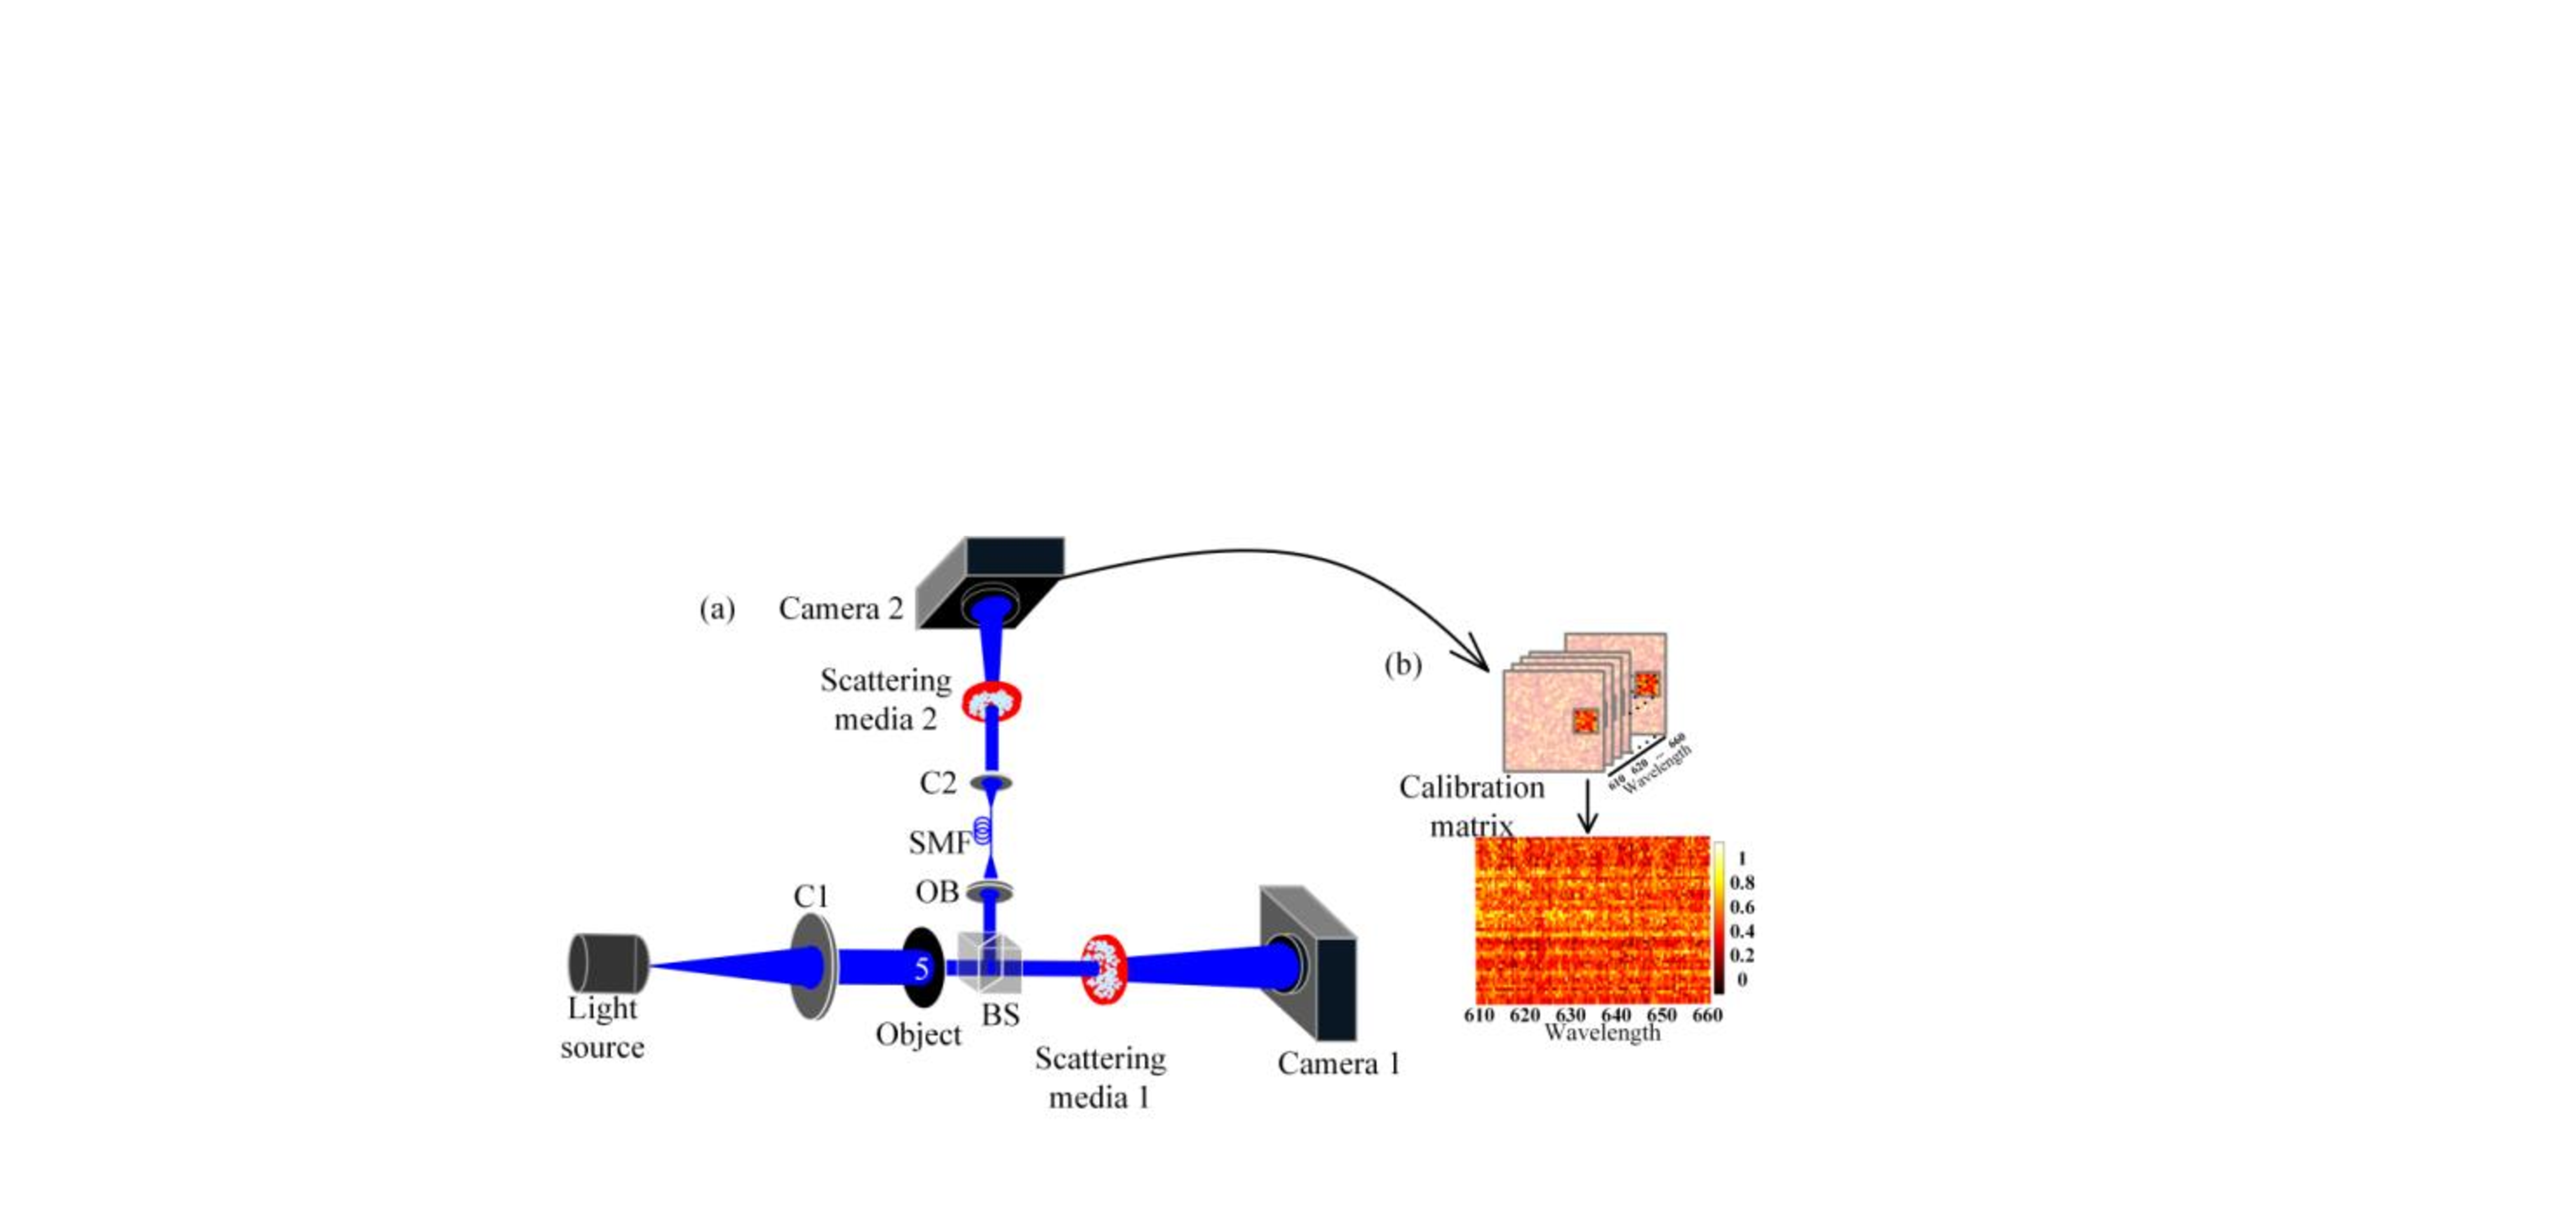
\includegraphics[scale=0.3]{Chapter3.FIG2.spectral_retrieval_model.pdf}
	\caption{透过散射介质的光谱信息和结构信息恢复的结构示意图}
	\label{fig:3.1}
\end{figure}

\subsection{基于光谱传输矩阵的光谱重建模型}
首先,我们需要引入散斑的光谱多样性概念。当特定波长以固定的角度照明散射介质时,在散射介质后固定位置处接受散斑图案。随着
\begin{figure}[htp]
	\centering
	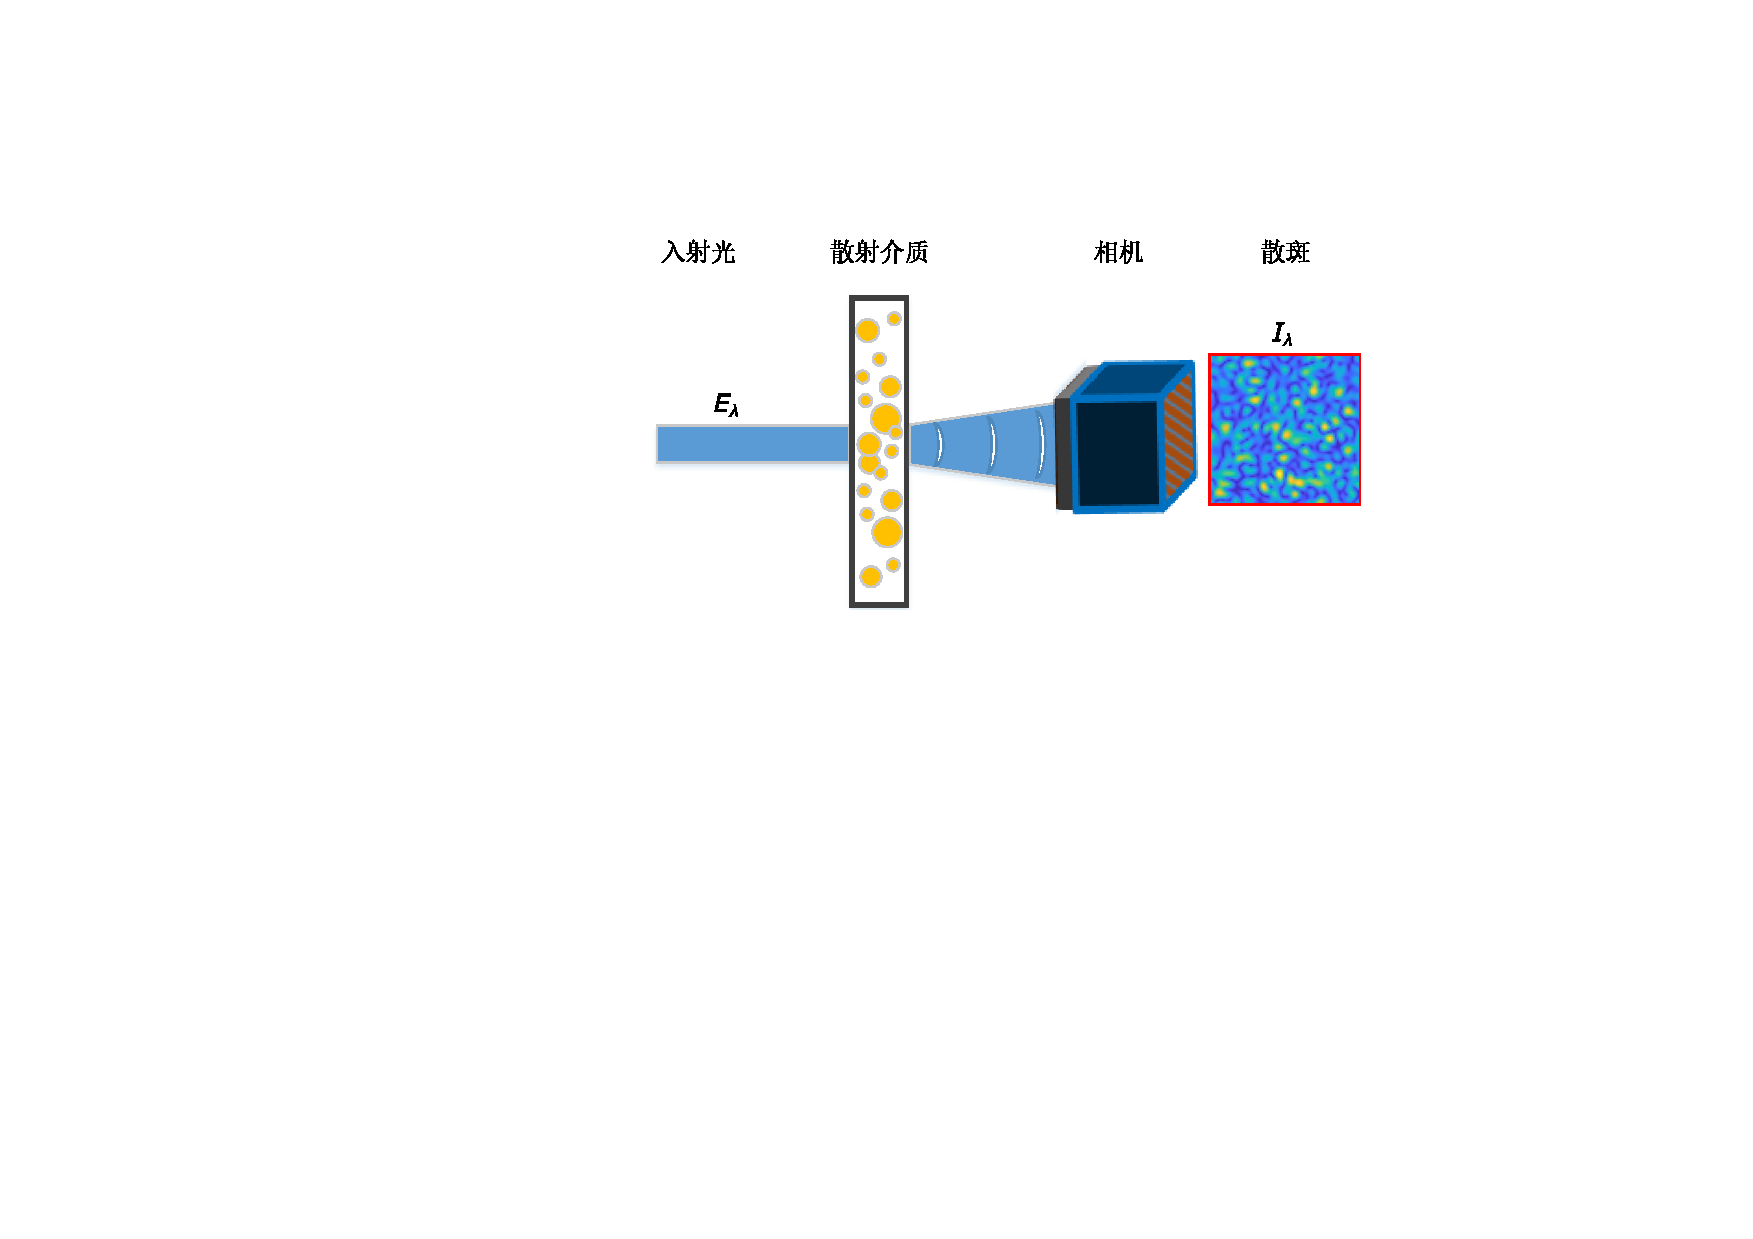
\includegraphics[scale=0.5]{C3.fig1.spectral_retrieval_model.pdf}
	\caption{透过散射介质的光谱信息和结构信息恢复的结构示意图}
	\label{fig:3.1}
\end{figure}

\section{声明}

声明是对学位论文创新性和使用授权的声明和说明,论文提交图书馆和存档时作者本人和指导教师必须签名确认。

声明部分标题字体为宋体,字号为四号加粗,居中排列,行距为固定值~20~磅,段落间距为段前~0~磅,段后~0~磅;正文字体为宋体,字号为小四号,行距为固定值~20~磅,段落间距为段前~0~磅,段后~0~磅;标题与正文之间空一行,签名行与正文之间空一行,日期行与签名行之间空一行。

\section{摘要}

摘要是学位论文的内容不加注释和评论的简短陈述,简明扼要陈述学位论文的研究目的、内容、方法、成果和结论,重点突出学位论文的创造性成果和观点。摘要包括中文摘要和英文摘要,硕士学位论文中文摘要字数一般为~1000~字左右,博士学位论文中文摘要字数一般为~1500~字左右。英文摘要内容与中文摘要内容保持一致,翻译力求简明精准。摘要的正文下方需注明论文的关键词,关键词一般为~3~ ~~8~个,关键词和关键词之间用逗号并空一格。

中文摘要标题字体为黑体,字号为三号,居中排列,行距为固定值~20~磅,段落间距为段前~24~磅,段后~18~磅;正文字体为宋体,字号为小四号,行距为固定值~20~磅,段落间距为段前~0~磅,段后~0~ 磅;关键词和正文之间空一行,关键词字体为宋体,字号为小四号,标题加粗。英文摘要标题字体为~Times New Roman~,字号为三号,居中排列,行距为固定值~20~磅,段落间距为段前~24~磅,段后~18~磅;正文的每一段落首行不空格,段落与段落之间空一行;正文字体为~Times New Roman~,字号为小四号,行距为固定值~20~磅,段落间距为段前~0~磅,段后~0~磅;关键词字体为~Times New Roman~,字号为小四号,标题加粗。

\section{插图索引}

学位论文中插图的目录索引。插图索引标题字体为黑体,字号为三号,居中排列,行距为固定值~20~磅,段落间距为段前~24~磅,段后~18~磅;正文内容字体为宋体,字号为小四号,行距为固定值~20~磅,段落间距为段前~0~磅,段后~0~磅。

\section{表格索引}

学位论文中表格的目录索引。表格索引标题字体为黑体,字号为三号,居中排列,行距为固定值~20~磅,段落间距为段前~24~磅,段后~18~磅;正文内容字体为宋体,字号为小四号,行距为固定值~20~磅,段落间距为段前~0~磅,段后~0~磅。

\section{符号对照表}

学位论文中符号代表的意义及单位(或量纲)的说明。符号对照表标题字体为黑体,字号为三号,居中排列,行距为固定值~20~磅,段落间距为段前~24~磅,段后~18~磅;正文内容字体为宋体,字号为小四号,行距为固定值~20~磅。

\section{缩略语对照表}

学位论文中缩略语代表意义的说明。缩略语按照英文单词首字母顺序排列,对照表标题字体为黑体,字号为三号,居中排列,行距为固定值~20~磅,段落间距为段前~24~磅,段后~18~磅;正文内容中文字体为宋体,字号为小四号,英文字体为~Times New Roman~,字号为小四号,行距为固定值~20~磅。

\section{目录}

目录是学位论文的提纲,是论文各组成部分的小标题,应分别依次列出并注明页码。各级标题分别以第一章、~1.1~、~1.1.1~等数字依次标出,目录中最多列出三级标题,正文中如果确需四级标题,用(1)、(2)形式标出。学位论文的前置部分(摘要、插图索引、表格索引、符号对照表、缩略语对照表)和学位论文的主体部分(正文、参考文献、致谢、作者简介)都要在目录中列出。

目录标题字体为黑体,字号为三号,居中排列,行距为固定值~20~磅,段落间距为段前~24~磅,段后~18~磅;目录内容中一级标题字体为黑体,字号为小四号,其余标题字体为宋体,字号为小四号。

\section{正文}

正文是学位论文的主体和核心部分。正文的一级标题居中排列,字体为黑体,字号为三号,行距为固定值~20~磅,段落间距为段前~24~磅,段后~18~磅;二级标题不缩进,字体为宋体加粗,字号为小三号,行距为固定值~20~磅,段落间距为段前~18~磅,段后~12~磅;三级标题缩进~2~ 字符,字体为宋体,字号为四号加粗,行距为固定值~20~磅,段落间距为段前~12~ 磅,段后~6~磅;正文内容字体为宋体,字号为小四号,行距为固定值~20~磅,段落间距为段前~0~磅,段后~0~磅。正文一般包括以下几个方面:

\subsection{绪论}

绪论是学位论文主体部分的开端,切忌与摘要雷同或成为摘要的注解。绪论除了要说明论文的研究目的、研究方法和研究结果外,还应评述与论文研究内容相关的国内外研究现状和相关领域中已有的研究成果;其次还要介绍本项研究工作的前提和任务、理论依据、实验基础、涉及范围、预期结果以及该论文在已有基础上所要解决的问题。

\subsection{各章节}

各章节一般由标题、文字叙述、图、表、公式等构成,章节内容总体要求立论正确,逻辑清晰,数据可靠,层次分明,文字通畅,编排规范。论文中若有与指导教师或他人共同研究的成果,必须明确标注;如果引用他人的结论,必须明确注明出处,并与参考文献保持一致。

(1)图:包括曲线图、示意图、流程图、框图等。图序号一律用阿拉伯数字分章依序编码,如:图~1.3~、图~2.11~。 每一个图应有简短确切的图名,连同图序号置于图的正下方。图名称、图中的内容字号为五号,中文字体为宋体,英文字体为~Times New Roman~,行距一般为单倍行距。图中坐标上标注的符号和缩略词必须与正文保持一致。引用图应在图题右上角标出文献来源;曲线图的纵横坐标必须标注“量、标准规定符号、单位”,这三者只有在不必要标明(如无量纲等)的情况下方可省略。

(2)表:包括分类项目和数据,一般要求分类项目由左至右横排,数据从上到下竖列。分类项目横排中必须标明符号或单位,竖列的数据栏中不要出现“同上”、“同左”等词语,一律要填写具体的数字或文字。表序号一律用阿拉伯数字分章依序编码,如:表~2.5~、表~10.3~。每一个表格应有简短确切的题名,连同表序号置于表的正上方。表名称、表中的内容字号为五号,中文字体为宋体,英文字体为~Times New Roman~,行距一般与正文保持一致。

(3)公式:正文中的公式、算式、方程式等必须编排序号,序号一律用阿拉伯数字分章依序编码,如:(3-32)、 (6-21)。对于较长的公式,另起行居中横排,只可在符号处(如:+、-、*、/、$<$$>$等)转行。公式序号标注于该式所在行(当有续行时,应标注于最后一行)的最右边。连续性的公式在“=”处排列整齐。大于~999~的整数或多于三位的小数,一律用半个阿拉伯数字符的小间隔分开;小于~1~的数应将~0~置于小数点之前。公式的行距一般为单倍行距。

(4)计量单位:学位论文中出现的计量单位一律采用国务院~1984~年~2~月~27~日发布的《中华人民共和国法定计量单位》标准。

\subsection{结论}

结论是学位论文最终和总体的结论,不是正文中各段的小结的简单重复,应准确、精炼、完整,其中要着重阐述作者研究的创造性成果以及在本研究领域中的重大意义,还可提出有待进一步研究和探讨的问题。

\section{参考文献}

参考文献是文中引用的有具体文字来源的文献集合,博士学位论文参考文献一般不少于~80~篇,其中近5年的参考文献不少于~20~篇,硕士学位论文参考文献一般不少于~30~篇,其中近5年的参考文献不少于~5~篇。参考文献标题字体为黑体,字号为三号,居中排列,段落间距为段前~24~磅,段后~18~磅;参考文献若是中文文献,字体为宋体,字号为五号,若是英文文献,字体为~Times New Roman~,字号为五号。学位论文的撰写要本着严谨求实的科学态度,凡有引用他人成果之处,引用处右上角用方括号标注阿拉伯数字编排的序号(必须与参考文献一致),同时所有引用的文献必须用全称,不能缩写,并按论文中所引用的顺序列于文末。引用文献的作者不超过~3~位时全部列出,超过时列前~3~位,后加“等”字或“et al.”。 参考文献的著录要符合《文后参考文献著录规则》(GB/T7714-2005)要求:

(1)期刊(报纸)参考文献:[序号] 主要责任者. 文献名称[文献类别代码]. 期刊(报纸)名, 年份, 卷(期): 引文页码.

(2)专著参考文献:[序号] 主要责任者. 专著名称[文献类别代码]. 其他责任者. 出版地: 出版单位, 出版年份.

(3)专利参考文献:[序号] 主要责任者. 专利名称: 国别, 专利号[文献类别代码]. 出版日期.

(4)技术标准参考文献:[序号] 起草责任者. 标准代号-标准顺序号-发布年. 标准名称[文献类别代码]. 出版地: 出版单位,出版年份.

(5)电子参考文献:[序号] 主要责任者. 题名[文献类别代码]. 获取和访问路径. [引用日期].

(6)会议论文集参考文献:[序号] 编者. 论文集名. (供选择项:会议名, 会址, 开会年)出版地: 出版者, 出版年份.

(7)学位论文参考文献:[序号]  主要责任者. 文献题名[文献类别代码]. 保存地: 保存单位, 年份.

(8)国际、国家标准参考文献:[序号] 标准代号. 标准名称[文献类别代码]. 出版地: 出版者, 出版年.

(9)报告类参考文献:[序号] 主要责任者. 文献题名[文献类别代码]. 报告地: 报告会主办单位, 年份.

参考文献著录中的文献类别代码:

(1)普通图书:M     \par
(2)会议录:C       \par
(3)汇编:G         \par
(4)报纸:N         \par
(5)期刊:J         \par
(6)学位论文:D     \par
(7)报告:R         \par
(8)标准:S         \par
(9)专利:P         \par
(10)数据库:DB     \par
(11)计算机程序:CP \par
(12)电子公告:EB   \par
载体类型:           \par
网络:OL             \par
磁带:MT             \par
磁盘:MK             \par
光盘:CD

\section{致谢}

作者对完成论文提供帮助和支持的组织和个人表示感谢的文字记载。致谢标题字体为黑体,字号为三号,居中排列,行距为固定值~20~磅,段落间距为段前~24~磅,段后~18~磅;正文内容字体为宋体,字号为小四号,行距为固定值~20~磅,段落间距为段前~0~磅,段后~0~磅。

\section{作者简介}

对作者的简要介绍,主要包括个人基本情况、教育背景、攻读博士/硕士学位期间的研究成果等三个部分内容。攻读博士/硕士学位期间的研究成果是指本人攻读博士/硕士学位期间发表(或录用)的学术论文,申请(授权)专利、参与的科研项目及科研获奖等情况,分别按时间顺序列出。其中,发表论文、申请(授权)专利、科研获奖只列出作者排名前~3~名的,参与的科研项目按重要程度最多列出~5~项。作者简介标题字体为黑体,字号为三号,居中排列,行距为固定值~20~ 磅,段落间距为段前~24~磅,段后~18~磅。作者简介的正文内容严格按照本模板中的范例书写。

\section{其他}

学位论文中如果需要注释,可作为脚注在页下分别著录,切忌在文中注释;如果有附录部分,可编写在正文之后,与正文连续编页码,每一附录均另页起,附录依次用大写英文字母~A、B、C……编序号,如:附录~A~、附录~B~等。
